\subsubsection{Généralités}

Les grands équipementiers comme CISCO proposent tous des solutions matérielles pour mettre en oeuvre des connexions VPN. Pour cette étude nous avons utilisé un routeur 2811XM adjoint des fonctionnalités de sécurité avancées fournies par la version \verb|c2800mn-advsecurityk9-mz.124-24.T.bin| de l'IOS.

Le choix d'IPsec s'est imposé comme solution naturelle, car très bien intégrée aux technologies CISCO. Ils proposent de plus un client IPsec multiplate-formes, permettent de gérer le processus d'authentification via certificats, et de s'interfacer à un annuaire d'identification en RADIUS.

\subsubsection{Mise en place côté serveur}

\paragraph{Configuration de base}
~

Commençons par configurer les interfaces du routeur. L'interface connectée au réseau de l'ISIMA récupère son adresse IP via DHCP ce qui ne serait pas le cas dans un environnement de production. En parallèle à cette configuration nous mettons en place deux ACL permettant de s'assurer sur seuls les clients du VPN pourront accéder au réseau interne.
% \begin{figure}[H]
	\begin{center}
		\begin{minipage}{0.90\textwidth}
			\begin{lstlisting}[frame=trBL]
(config)# hostname CISCOVPN
(config)# enable secret cisco
(config)# no ip domain-lookup
(config)# access-list 1 permit 10.0.1.0 0.0.0.255
(config)# access-list 2 permit 192.168.1.0 0.0.0.255
(config)# interface FastEthernet0/0
(config-if)# description interface to the external network
(config-if)# ip address dhcp
(config-if)# no shutdown
			\end{lstlisting}
		\end{minipage}
	\end{center}
\begin{figure}[H]
	\begin{center}
		\begin{minipage}{0.90\textwidth}
			\begin{lstlisting}[frame=trBL]
(config-if)# exit
(config)# interface FastEthernet0/1.1
(config-if)# description interface to the prof network
(config-if)# encapsulation dot1Q 333
(config-if)# ip address 10.0.0.1 255.255.255.0
(config-if)# ip access-group 1 out
(config-if)# exit
(config)# interface FastEthernet0/1.2
(config-if)# description interface to the student network
(config-if)# encapsulation dot1Q 111
(config-if)# ip address 192.168.0.1 255.255.255.0
(config-if)# ip access-group 2 out
(config-if)# exit
(config)# interface FastEthernet0/1
(config-if)# no shutdown
(config-if)# exit
			\end{lstlisting}
		\end{minipage}
	\end{center}
	\caption{Configuration des interfaces}
	\label{configuration_interfaces}
\end{figure}

~

Configurons maintenant les accès à distance au routeur :
\begin{figure}[H]
	\begin{center}
		\begin{minipage}{0.95\textwidth}
			\begin{lstlisting}[frame=trBL]
(config)# banner login #Unauthorized access prohibited - F5 only!#
(config)# banner motd #
This router is part of a wonderfull ZZ3F5 project for 2008-2009.
If you have any question, comment, insults, whatsoever...
please contact coscia@poste.isima.fr and dessaux@poste.isima.fr.
Thank you if you read this till the end.#
(config)# enable secret cisco
(config)# line con 0
(config-line)# logging synchronous
(config-line)# password cisco
(config-line)# login
(config-line)# exit
(config)# line vty 0 4
(config-line)# transport input telnet
(config-line)# password cisco
(config-line)# login
(config-line)# exit
(config)# service password-encryption
			\end{lstlisting}
		\end{minipage}
	\end{center}
	\caption{Configuration de l'accès à distance}
	\label{configuration_acces_a_distance}
\end{figure}

\paragraph{Configuration de l'authentification Radius}
\label{CONFIG_RADIUS}
~

Dans cette section nous allons interfacer le routeur avec un serveur RADIUS. Pour installer ce serveur nous allons tirer parti du serveur \verb|Linux CentOS 5.1| qui est déjà capable de récupérer les identifiants via l'annuaire NIS de l'ISIMA.

Le serveur à installer est FreeRadius, qui est disponible dans les paquets de la distribution :

\verb|[root@centosvpn ~]# yum install freeradius|

~

La configuration de base de FreeRadius étant déjà fonctionnelle nous n'auront que très peu de modifications à lui apporter. Tout d'abord nous allons configurer une authentification PAP entre le routeur et le serveur Radius, en ajoutant \verb|ciscovpn User-Password := "isima"|  au début du fichier \verb|/etc/raddb/users|, où ciscovpn est le hostname du routeur et isima le mot de passe qui lui sera associé.

Nous allons ensuite autoriser le routeur à se connecter en ajoutant les lignes suivantes dans le fichier \verb|/etc/raddb/clients.conf|, en supposant que \verb|192.168.102.86| est l'adresse IP du routeur sur le réseau de l'ISIMA :
\begin{center}
		\begin{minipage}{0.9\textwidth}
			\begin{lstlisting}[frame=trBL]
client 192.168.102.86 {
	secret = isima
	shortname = isima
}
			\end{lstlisting}
		\end{minipage}
\end{center}
~

Il reste à indiquer au Radius qu'il doit interroger la base NIS pour obtenir les identifiants et mots de passes utilisateurs. Cela se fait en commentant la ligne indiquant à FreeRadius le chemin vers le fichier \verb|shadow| dans le fichier \verb|/etc/raddb/radiusd.conf|. En effet, en l'absence de fichier \verb|shadow|, FreeRadius se rabat sur les mécanismes d'authentification PAM standarts dont nous avons besoin.

~

Du point de vue du routeur, le protocole RADIUS étant parfaitement géré par les équipements CISCO la configuration qui en découle est relativement simple :

\begin{figure}[H]
	\begin{center}
		\begin{minipage}{0.90\textwidth}
			\begin{lstlisting}[frame=trBL]
(config)# aaa new-model
(config)# radius-server host 192.168.102.121 auth-port 1812
acct-port 1813 key isima
(config)# ip radius source-interface FastEthernet 0/0
(config)# aaa group server radius RadiusServer
(config-sg-radius)# radius-server host 192.168.102.121 auth-port
1812 acct-port 1813
(config-sg-radius)# exit
(config)# aaa authentication login default group RadiusServer
			\end{lstlisting}
		\end{minipage}
	\end{center}
	\caption{Configuration de l'authentification Radius}
	\label{configuration_authentification_radius}
\end{figure}


\paragraph{Configuration d'IPsec}
~

Les lignes qui suivent permettent de configurer la cryptographie isakmp comme suit :
\begin{itemize}
	\item algorithme de chiffrement triple DES.
	\item algorithme de hashage sha-1.
	\item authentification via clefs partagées.
	\item Diffie-Hellman 1024 bits.
	\item durée de vie du contexte cryptographique égale à une journée.
	\item utilisation du hostname plutôt que de l'adresse IP pour protéger les échanges.
\end{itemize}


\begin{figure}[H]
	\begin{center}
		\begin{minipage}{0.90\textwidth}
			\begin{lstlisting}[frame=trBL]
(config)# crypto isakmp policy 1
(config-isakmp)# encryption 3des
(config-isakmp)# hash sha
(config-isakmp)# authentication pre-share
(config-isakmp)# group 2
(config-isakmp)# lifetime 86400
(config-isakmp)# exit
(config)# crypto isakmp identity hostname
			\end{lstlisting}
		\end{minipage}
	\end{center}
	\caption{Configuration IKE}
	\label{configuration_ike}
\end{figure}

Ajoutons les pools DHCP qui fourniront leurs adresses IP aux étudiants et aux professeurs :
\begin{figure}[H]
	\begin{center}
		\begin{minipage}{0.90\textwidth}
			\begin{lstlisting}[frame=trBL]
(config)# ip local pool profs 10.0.1.20 10.0.1.254
(config)# crypto isakmp client configuration group profs
(config-isakmp-group)# key isimaprofs
(config-isakmp-group)# dns 10.0.0.11
(config-isakmp-group)# domain isima.fr
(config-isakmp-group)# pool profs
(config-isakmp-group)# exit

(config)# ip local pool students 192.168.1.20 192.168.1.254
(config)# crypto isakmp client configuration group students
(config-isakmp-group)# key isimastudents
(config-isakmp-group)# dns 192.168.1.11
(config-isakmp-group)# domain isima.fr
(config-isakmp-group)# pool students
(config-isakmp-group)# exit
			\end{lstlisting}
		\end{minipage}
	\end{center}
	\caption{Configuration des pools utilisateurs}
	\label{configuration_pools_utilisateurs}
\end{figure}


Configurons maintenant la police IPsec :
\begin{itemize}
	\item Mise en place de l'ACL pour indiquer que l'on veut filtrer l'ensemble du trafic IP.
	\item Encapsulation ESP, chiffrement 3des, intégrité sha-1.
% 	\item Mode tunnel (ie au niveau 3, par opposition au mode transport au niveau 4).
	\item Configuration de l'authentification des profs et des étudiants via le serveur radius.
\end{itemize}

\begin{figure}[H]
	\begin{center}
		\begin{minipage}{1\textwidth}
			\begin{lstlisting}[frame=trBL]
(config)# access-list 101 permit ip any any
(config)# crypto ipsec transform-set policy esp-3des esp-sha-hmac
(cfg-crypto-trans)# exit
(config)# crypto dynamic-map prof-map 1
(config-crypto-map)# set transform-set policy
(config-crypto-map)# exit

(config)# crypto map prof-map
(config)# crypto map prof-map 1 ipsec-isakmp dynamic prof-map
(config)# crypto map prof-map client authentication list RadiusServer
(config)# crypto map prof-map client configuration address respond
(config)# crypto map prof-map isakmp authorization list 101

(config)# aaa authorization network 101 local
			\end{lstlisting}
		\end{minipage}
	\end{center}
	\caption{Configuration de la police IPsec}
	\label{configuration_police_ipsec}
\end{figure}

La présence d'une authentification en fonction de groupes protégés via une clef partagée est une lacune sécuritaire de notre solution. En effet un étudiant pourrait ``facilement'' se faire passer pour un professeur. Pour remédier à ce problème un mécanisme d'authentification via certificats est nécessaire.

Nous allons utiliser le service Windows 2003 SCEP installé dans la partie 2.1.1.\ref{autorité_certification} page \pageref{autorité_certification}. La figure \ref{configuration_authentification_certificats} détaille la configuration d'une authentification par certificats sur le routeur. Lors de la requête de certificat, un mot de passe permettant de vérifier la validité de la demande est demandé : il se trouve à l'adresse \verb|http://192.168.102.250/certsrv/mscep/mscep.dll|

\begin{figure}[H]
	\begin{center}
		\begin{minipage}{1\textwidth}
			\begin{lstlisting}[frame=trBL]
(config)# crypto ca identity isima.fr
(ca-trustpoint)# enrollment url
http://192.168.102.250/certsrv/mscep/mscep.dll
(ca-trustpoint)# exit
(config)# crypto ca authenticate isima.fr
(config)# crypto ca trustpoint isima.fr
(ca-trustpoint)# crl optional
(ca-trustpoint)# exit
(config)# crypto isakmp policy 1
(config-isakmp)# authentication rsa-sig
(config-isakmp)# exit
			\end{lstlisting}
		\end{minipage}
	\end{center}
	\caption{Configuration de l'authentification via certificats}
	\label{configuration_authentification_certificats}
\end{figure}

Il ne reste plus qu'à attendre la validation (manuelle!) de la demande de certificat par l'administrateur du serveur jouant le rôle de l'autorité de certification.

\subsubsection{Mise en place côté client}

Cette partie présente l'installation du client CISCO sur une machine Windows. Bien que ce client aie la particularité d'être compatible avec Linux nous ne sommes pas parvenus, ni à la compiler (il réclame la compilation d'un module noyau), ni à nous en servir.

L'installation du client est comme pour n'importe quel logiciel sous Windows. Une fois lancé il faut établir une nouvelle connexion (bouton ``new''). La figure \ref{VPN_CISCO} présente les informations nécessaires à la connexion : legroupe d'appartenance du client, l'adresse IP du serveur et la clé partagé.

\begin{figure}[H]
	\begin{center}
		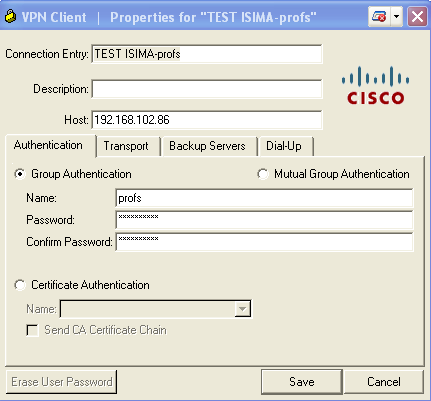
\includegraphics[width=0.6\textwidth]{partie_2/screen_windows/client_cisco.png}\\
	\end{center}
	\caption{Client CISCO}
	\label{VPN_CISCO}
\end{figure}

Si la configuration est correcte, lorsque l'utilisateur tentera de se connecter au VPN il se verra demander ses identifiant et mot de passe, correspondant à ceux inscrits dans l'annuaire de l'ISIMA :

\begin{figure}[H]
	\begin{center}
		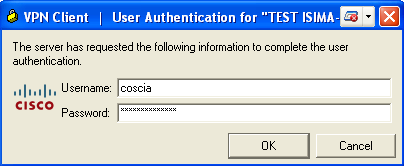
\includegraphics[width=0.5\textwidth]{partie_2/screen_windows/fenetre_connexion.PNG}\\
	\end{center}
	\caption{Identification du client}
	\label{VPN_CISCO_CLIENT}
\end{figure}

\subsubsection{Bilan et limites de la solution}

% Dans cette partie, nous ferons des brefs tests de connexion afin de vérifier le bon fonctionnement de la solution.
% 
% 
% \begin{figure}[H]
% 	\begin{center}
% 		\begin{minipage}{1\textwidth}
% 			\begin{lstlisting}[frame=trBL]
% 
% 
% Configuration IP de Windows
% 
% Carte Ethernet Connexion au réseau local:
% 
%         Suffixe DNS propre à la connexion : isima.fr
% 	Adresse IP. . . . . . . . . . . . : 192.168.102.79
% 	Masque de sous-réseau . . . . . . : 255.255.255.0
% 	Passerelle par défaut . . . . . . : 192.168.102.60
% 
% 
% Carte Ethernet Connexion au réseau local 3:
% 
%         Suffixe DNS propre à la connexion : isima.fr
% 	 Adresse IP. . . . . . . . . . .  : 10.0.1.22
% 	Masque de sous-réseau . . . . . . : 255.0.0.0
% 	Passerelle par défaut . . . . . . : 10.0.1.22
% 
% 
% 			\end{lstlisting}
% 		\end{minipage}
% 	\end{center}
% 	\caption{Adresse IP coté profs}
% 	\label{Adresse_IP_cote_profs}
% \end{figure}
% 
% 
% On peut refaire la même expérience en se connectant avec un utilisateur appartenant au groupe STUDENTS.
% 
% \begin{figure}[H]
% 	\begin{center}
% 		\begin{minipage}{1\textwidth}
% 			\begin{lstlisting}[frame=trBL]
% 
% 
% Configuration IP de Windows
% 
% Carte Ethernet Connexion au réseau local:
% 
%         Suffixe DNS propre à la connexion : isima.fr
% 	Adresse IP. . . . . . . . . . . . : 192.168.102.79
% 	Masque de sous-réseau . . . . . . : 255.255.255.0
% 	Passerelle par défaut . . . . . . : 192.168.102.60
% 
% 
% Carte Ethernet Connexion au réseau local 3:
% 
%         Suffixe DNS propre à la connexion : isima.fr
%        
% 	 Adresse IP. . . . . . . . . . .  : 192.168.1.20
% 	Masque de sous-réseau . . . . . . : 255.255.255.0
% 	Passerelle par défaut . . . . . . : 192.168.1.20
% 
% \end{lstlisting}
% 		\end{minipage}
% 	\end{center}
% 	\caption{Adresse IP coté eleve}
% 	\label{Adresse_IP_cote_eleve}
% \end{figure}

% On remarque bien que la solution CISCO est fonctionnelle, en fonction du groupe d'appartenance le routeur est capable de rediriger l'utilisateur sur le bon réseau.

La phase de configuration du routeur a tiré sa difficulté de la complexité inhérente à IPsec. Cette complexité impose de suivre l'ensemble des étapes qui nous avons détaillées ``à la lettre'' afin de valider par étapes les paramètres de chaque élément constitutif d'IPsec.

L'aspect sécurité est très présent, étant la raison d'être d'IPsec. En effet, dès le début de la phase d'authentification, l'ensemble des échanges est chiffré. Le principal problème que nous avons rencontré concerne le mécanisme d'authentification. En effet, le système en place sur la solution n'est qu'un système à clef partagée car nous ne sommes pas parvenus à aller au bout de la mise en place des certificats. En effet nous avons été capables de fournir des certificats signés par notre autorité au routeur comme au client, néanmoins la connexion n'a jamais pu être établie.
